\chapter{Experiments} \label{chap:experiments}

The developed framework presented and described in Chapter~\ref{chap:framework} obligate to the validation of each module in order to assure consistency and robustness in the results that such system produced. Having this considered, we stipulate several experiments, in which each of them was related to a specific task. 

\section*{}

\section{Exploratory Data Analysis}\label{sec:exploratory_data_analysis}

The main goal of this section is the devise of relevant analysis taking into consideration the five different collected datasets. Since this dissertation is supported in experiments using real-world data, such analysis is crucial in order to gain better knowledge of the intrinsic characteristics of it. A tweet provides some fields of interest, such as, the text message, date of creation, language, and the \emph{entities}, which are constantly analysed in several data analytics systems. An \emph{entity} is metadata and additional contextual information contained in the tweet and is composed by the \emph{hashtags}, \emph{user mentions}, \emph{urls} and \emph{media} fields. We count the amount of tweets containing this kind of information for all the cities, London, New York, Melbourne, Rio de Janeiro and São Paulo, and projected some data visualizations for different temporal frequencies. The following subsections are divided into three different categories:  (1) Geographical Distribution, (2) Temporal Frequencies and (3) Metadata Composition. Additionally, we discuss the results of each city, as well as the main observable differences.

\subsection{Geographic Distributions}

The bounding-boxes selected to perform the data collection had its origin in an open-sourced tool 

\begin{figure}[h]
    \centering
    \begin{subfigure}[t]{0.31\textwidth}
        \centering
        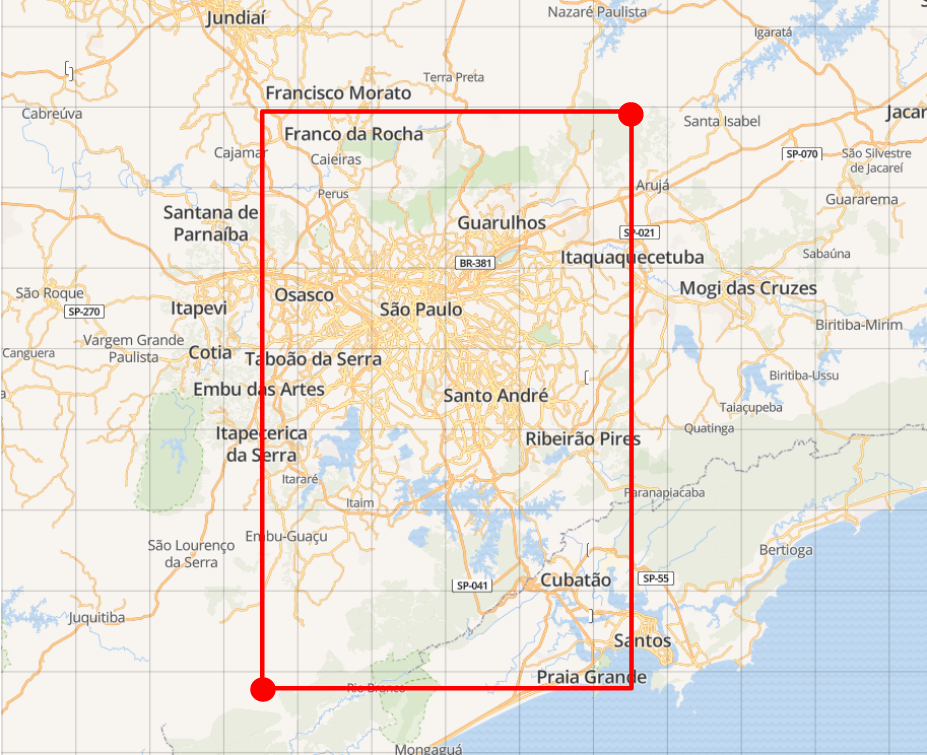
\includegraphics[width=1\linewidth]{figures/sp_bb.png}
        \caption{São Paulo}
        \label{fig:saopaulo_bounding_box}
    \end{subfigure}%
    \quad
    \begin{subfigure}[t]{0.3\textwidth}
        \centering
        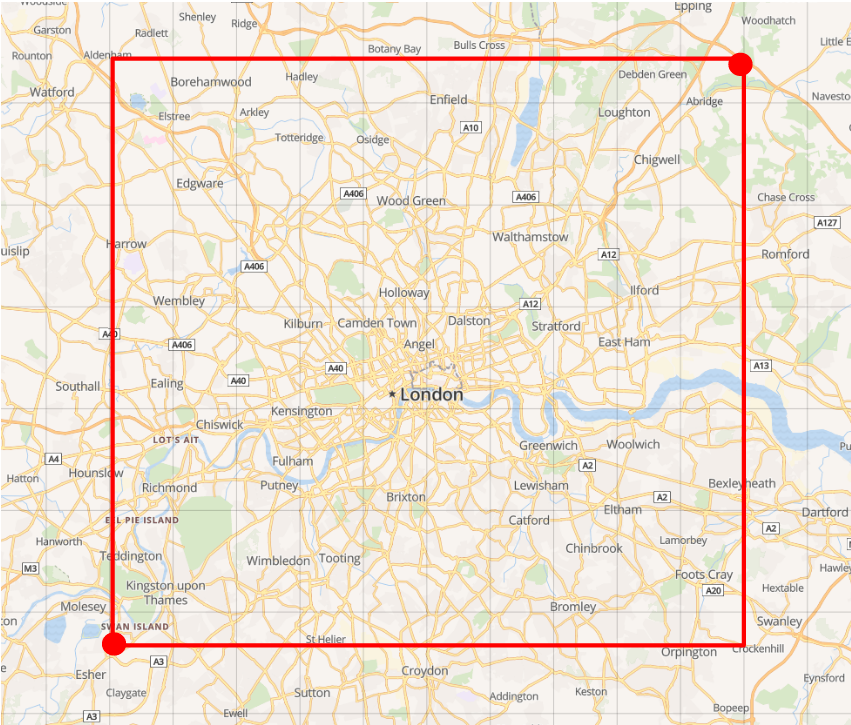
\includegraphics[width=1\linewidth]{figures/london_bb.png}
        \caption{London}
        \label{fig:london_bounding_box}
    \end{subfigure}
    \quad
    \begin{subfigure}[t]{0.3\textwidth}
        \centering
        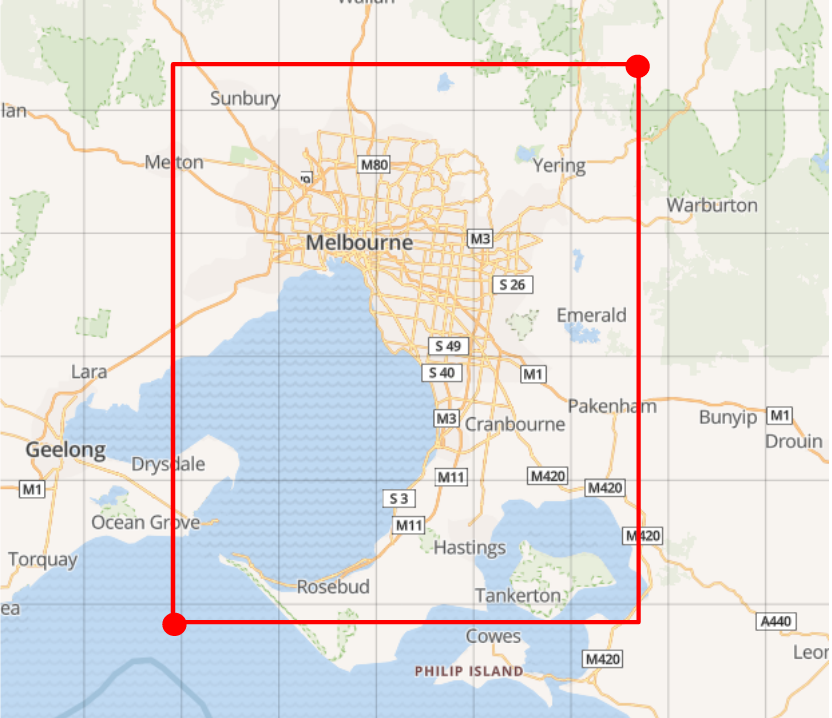
\includegraphics[width=1\linewidth]{figures/melbourne_bb.png}
        \caption{Melbourne}
        \label{fig:melbourne_bounding_box}
    \end{subfigure}
    
    \medskip
    
     \begin{subfigure}[t]{0.42\textwidth}
        \centering
        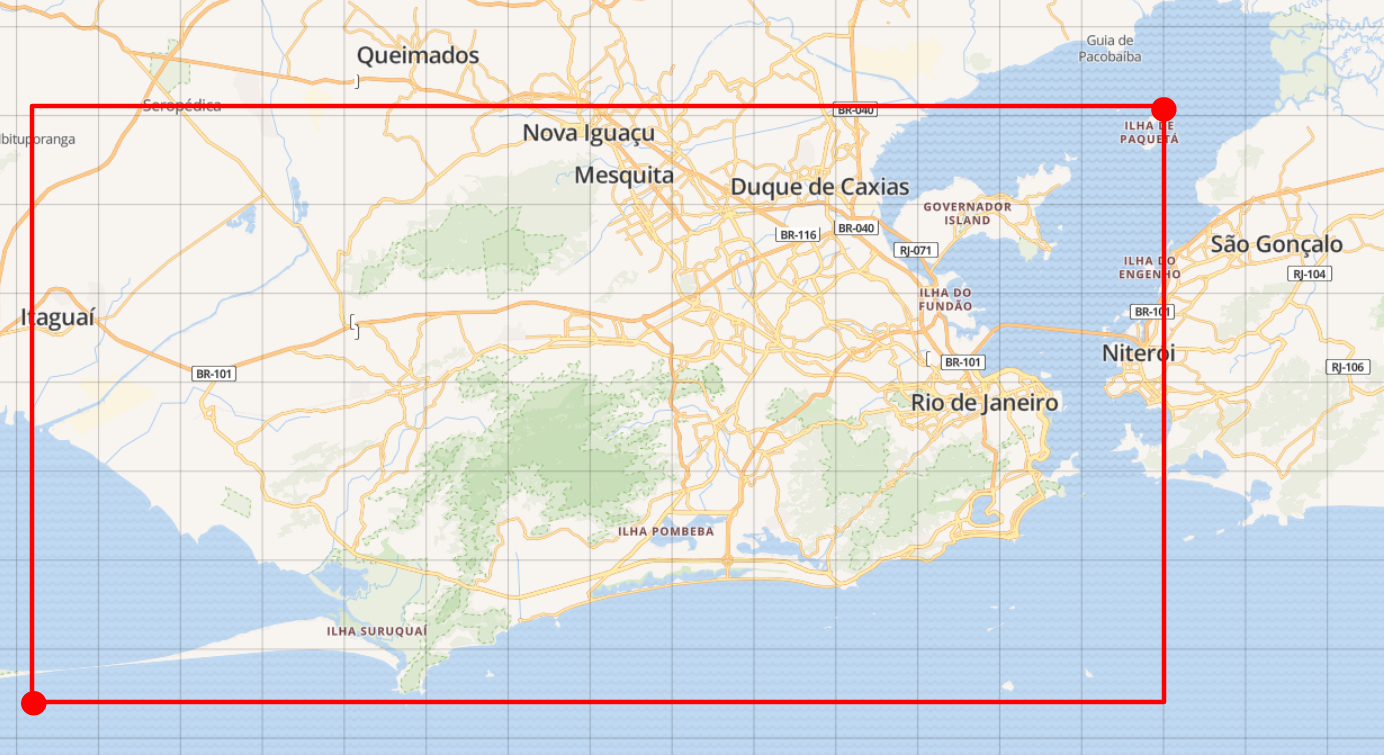
\includegraphics[width=1\linewidth]{figures/rio_bb.png}
        \caption{Rio de Janeiro}
        \label{fig:riodejaneiro_bounding_box}
    \end{subfigure}
    \quad
    \begin{subfigure}[t]{0.38\textwidth}
        \centering
        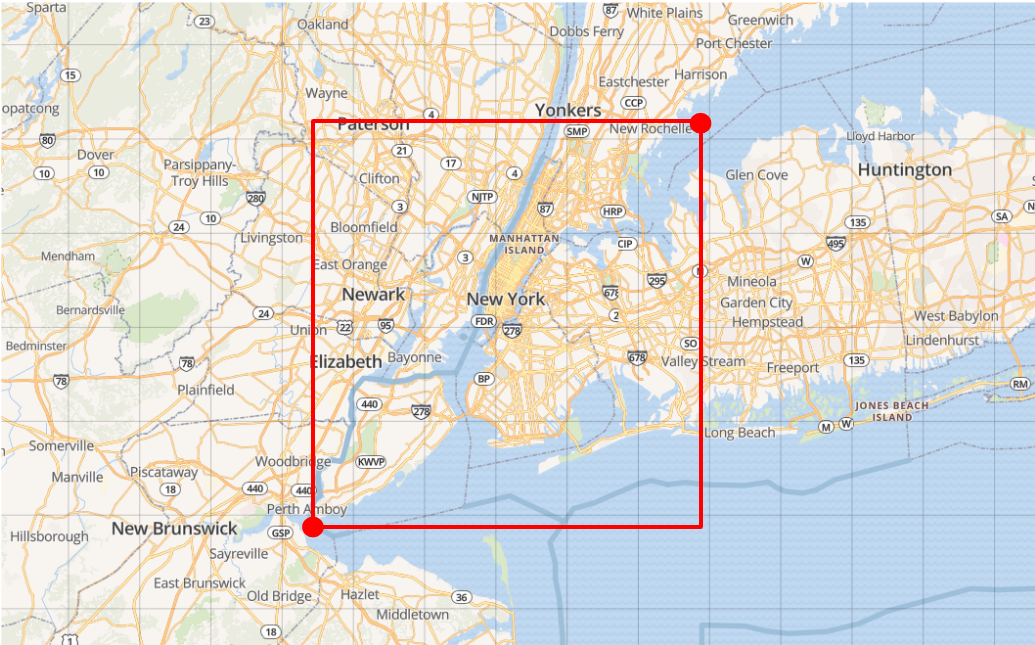
\includegraphics[width=1\linewidth]{figures/newyork_bb.png}
        \caption{New York}
        \label{fig:newyork_bounding_box}
    \end{subfigure}
    \caption{Search Bounding-boxes for the data collection}
    \label{fig:bounding_boxes}
\end{figure}

\subsection{Temporal Frequencies}

\begin{figure}[h]
    \centering
    \begin{subfigure}[t]{0.45\textwidth}
        \centering
        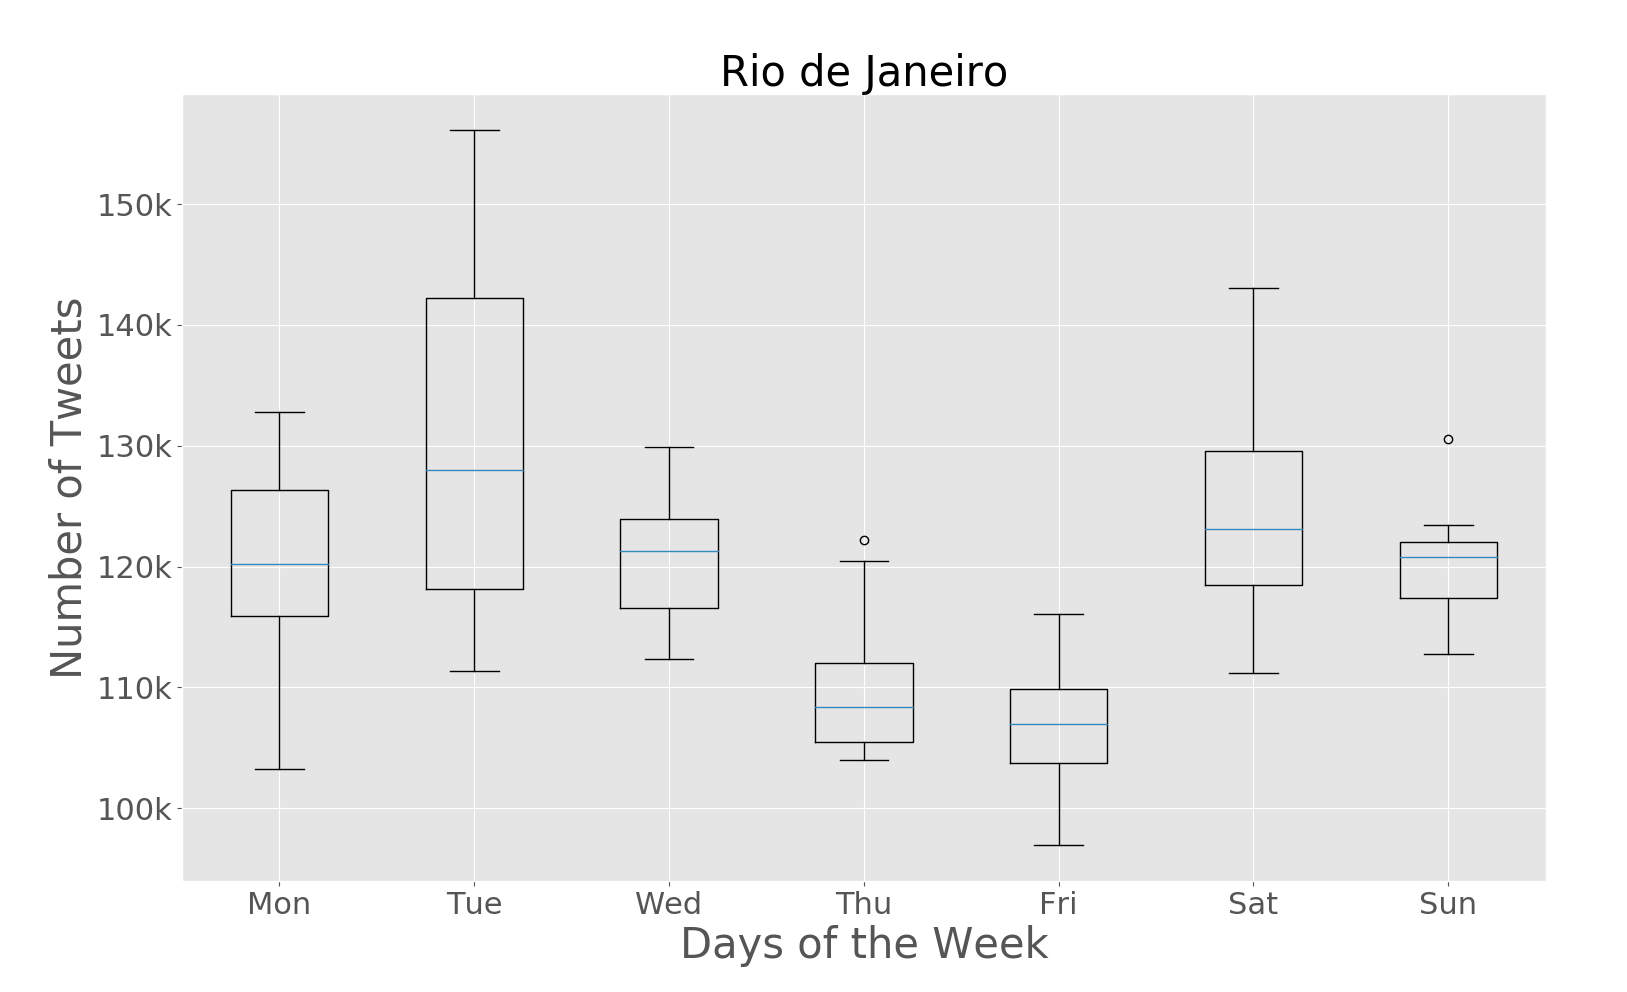
\includegraphics[width=1\linewidth]{figures/rio_box_plt_day_of_week.png}
        \caption{}
        \label{fig:riodejaneiro_box_plot_day_of_week}
    \end{subfigure}%
    \quad
    \begin{subfigure}[t]{0.45\textwidth}
        \centering
        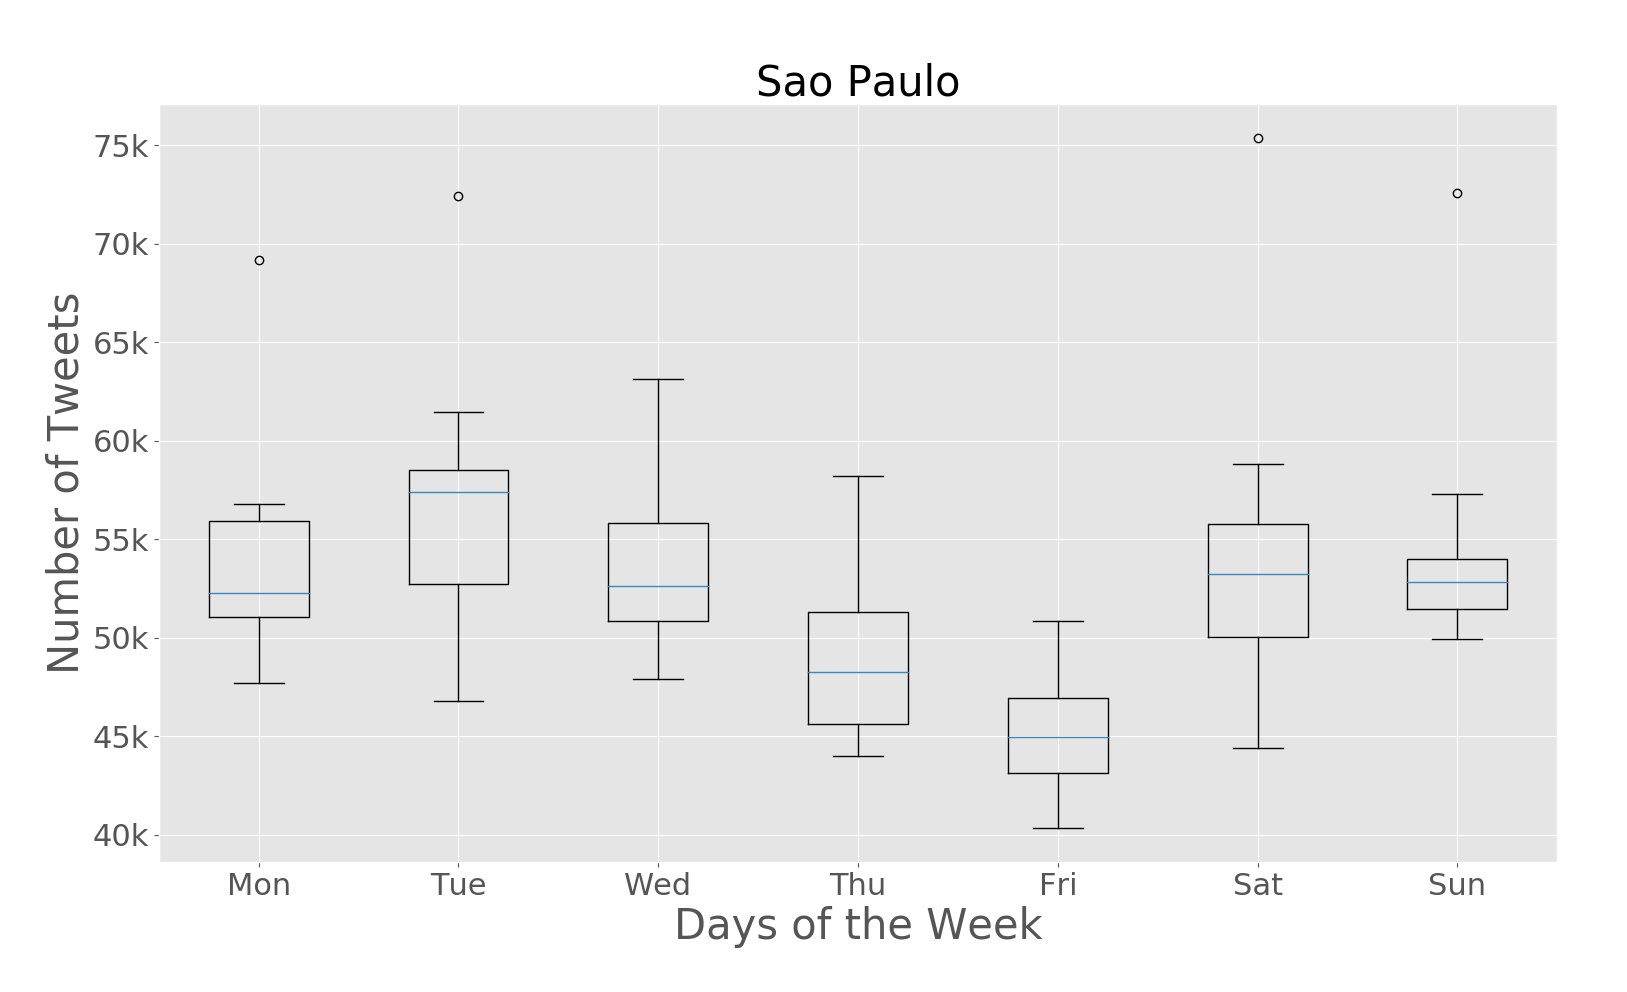
\includegraphics[width=1\linewidth]{figures/sp_box_plt_day_of_week.png}
        \caption{}
        \label{fig:saopaulo_box_plot_day_of_week}
    \end{subfigure}

    \medskip

    \begin{subfigure}[t]{0.45\textwidth}
        \centering
        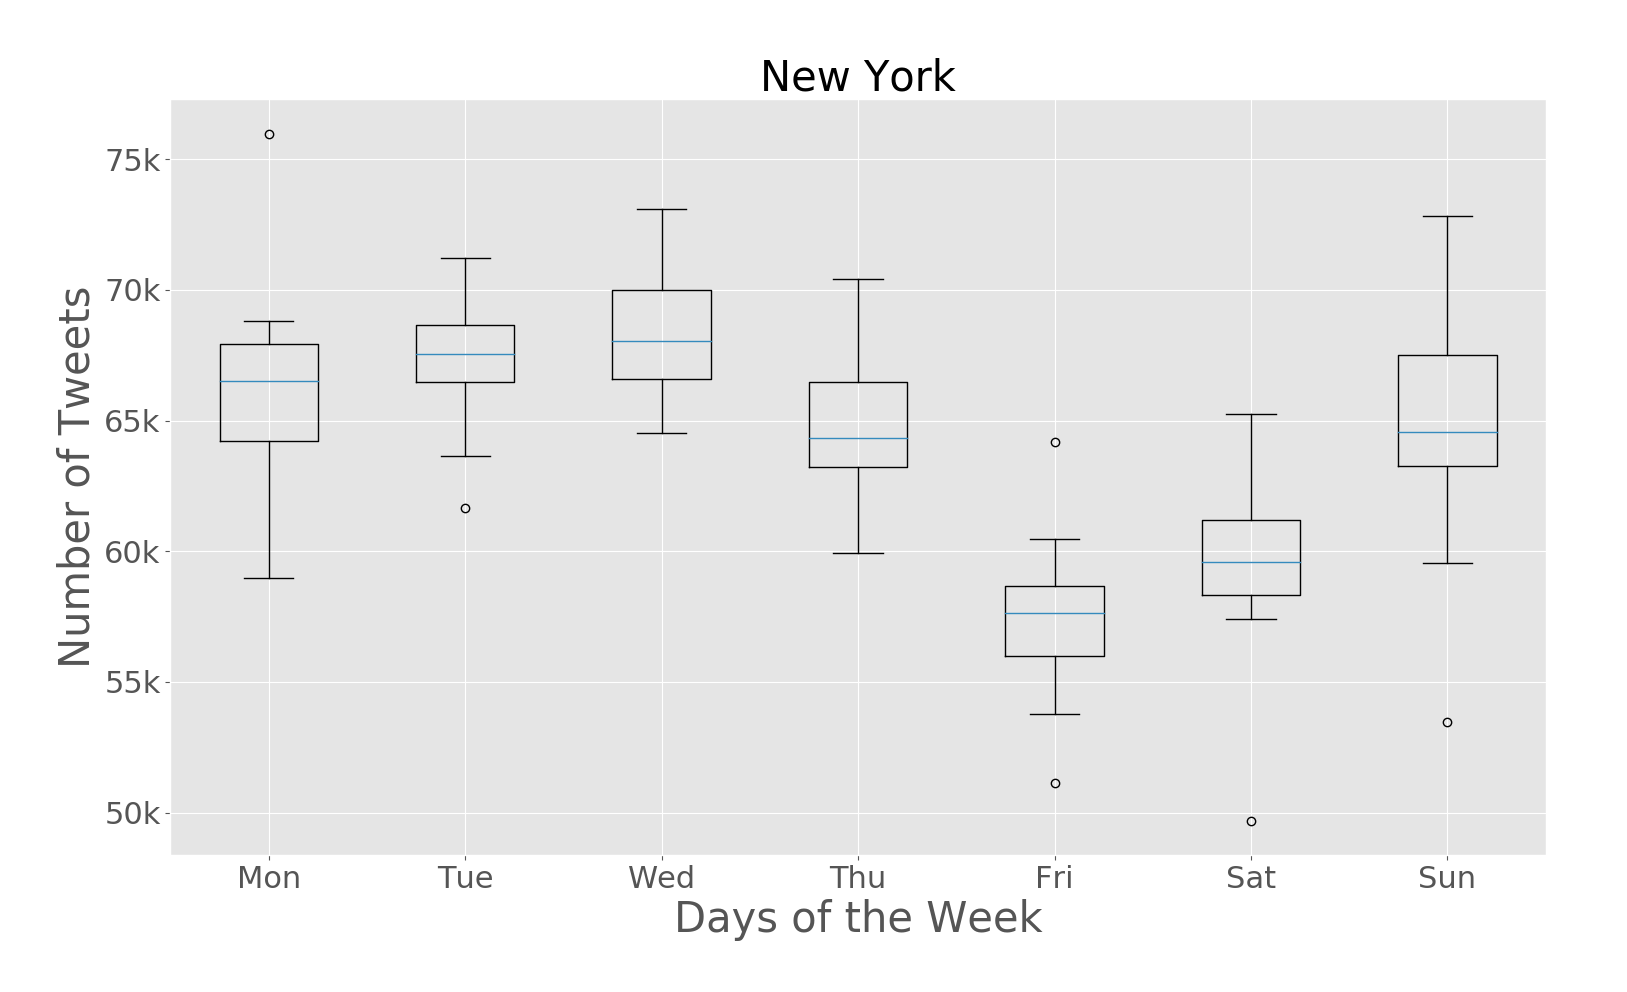
\includegraphics[width=1\linewidth]{figures/nyc_box_plt_day_of_week.png}
        \caption{}
        \label{fig:newyork_box_plot_day_of_week}
    \end{subfigure}
    \quad
    \begin{subfigure}[t]{0.45\textwidth}
        \centering
        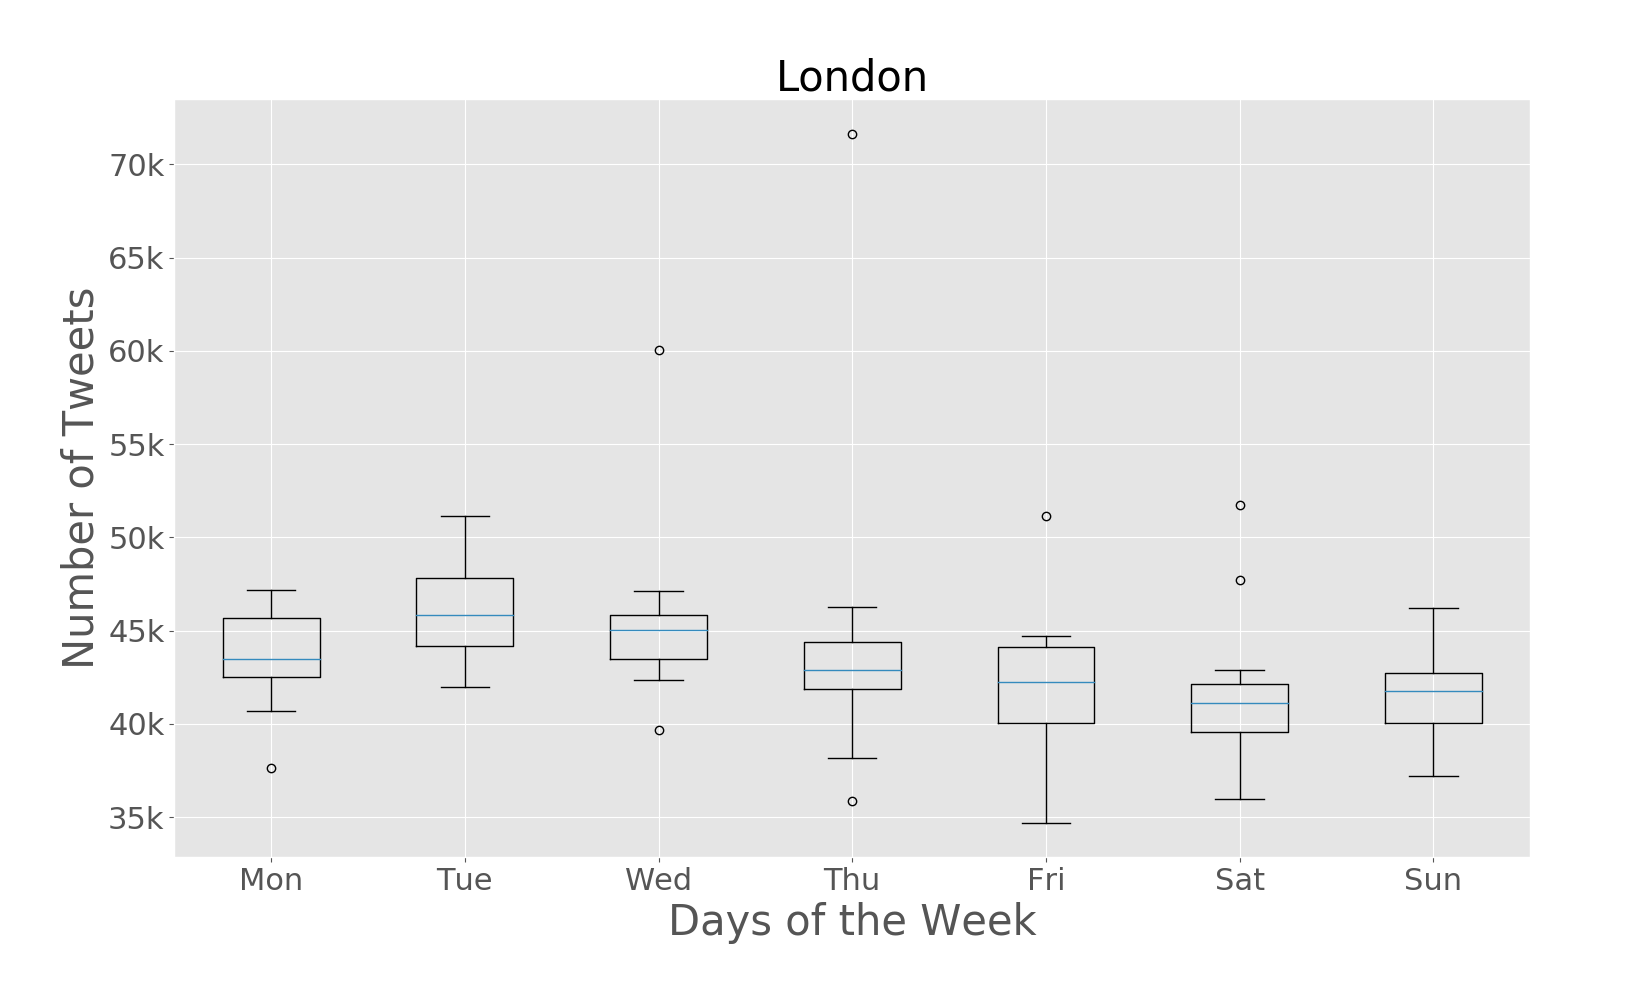
\includegraphics[width=1\linewidth]{figures/london_box_plt_day_of_week.png}
        \caption{}
        \label{fig:london_box_plot_day_of_week}
    \end{subfigure}

	\medskip
    
     \begin{subfigure}[t]{0.45\textwidth}
        \centering
        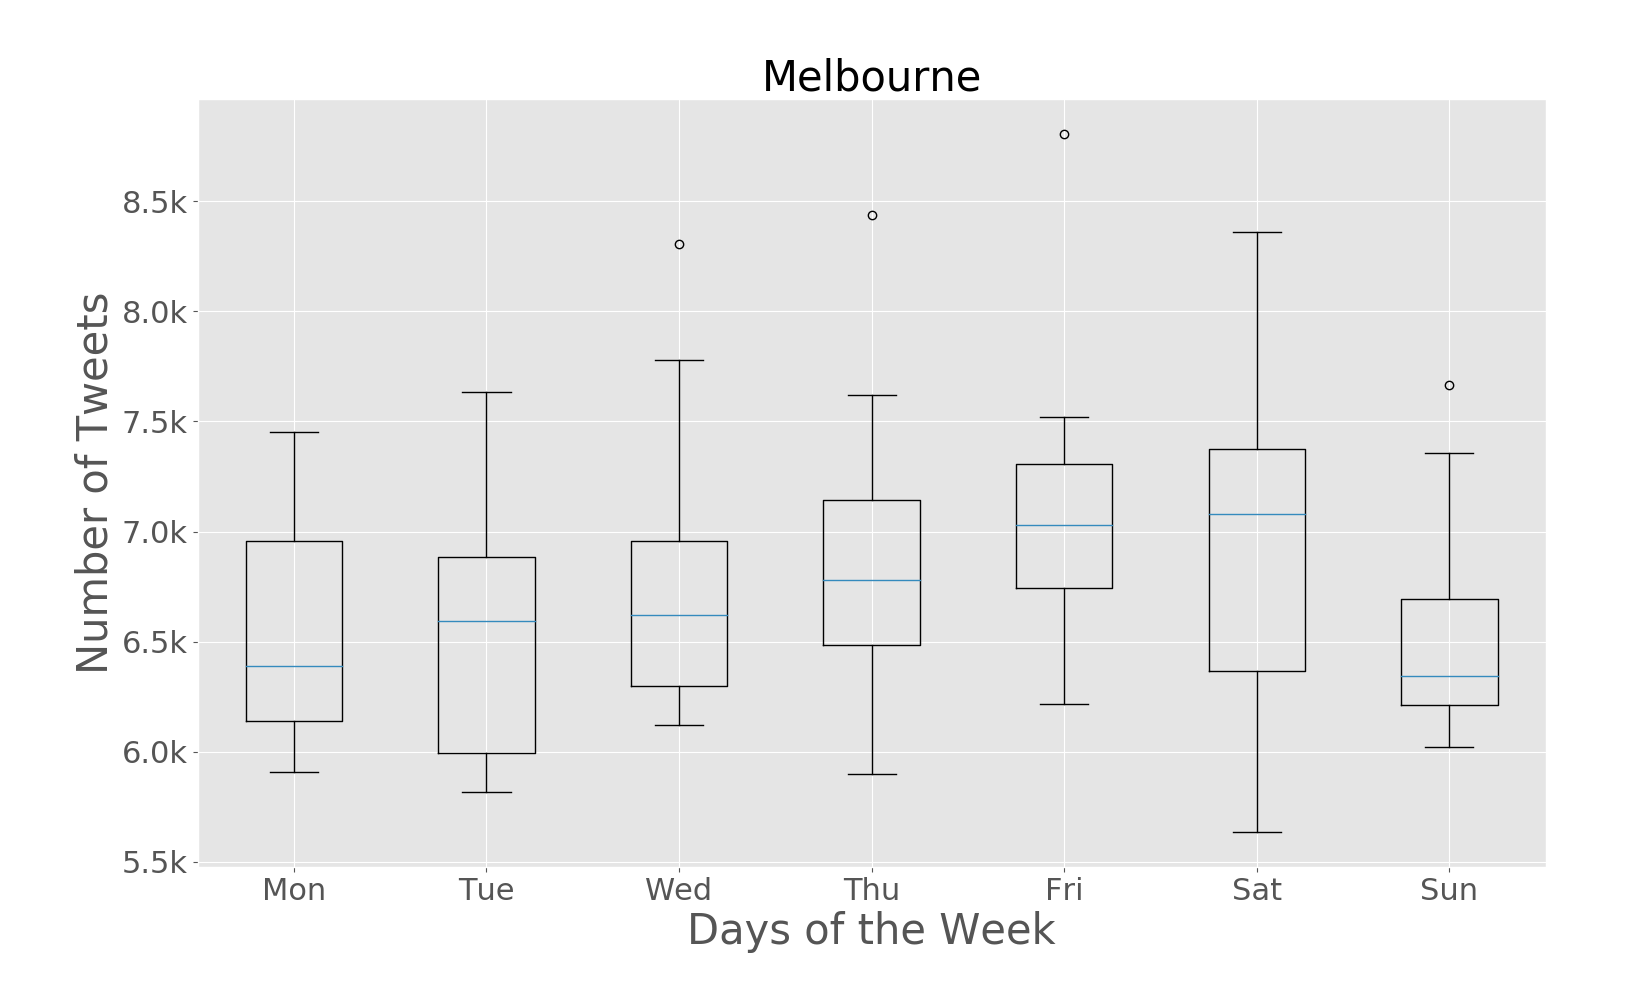
\includegraphics[width=1\linewidth]{figures/melbourne_box_plt_day_of_week.png}
        \caption{}
        \label{fig:melbourne_box_plot_day_of_week}
    \end{subfigure}
    
\caption[Five numerical solutions]{Days-of-the-week box-plots for the volume of tweets (a) Rio de Janeiro (b) São Paulo (c) New York City (d) London (e) Melbourne}
\end{figure}

\begin{figure}[htbp]
\centering
   \begin{subfigure}[t]{\textwidth}
   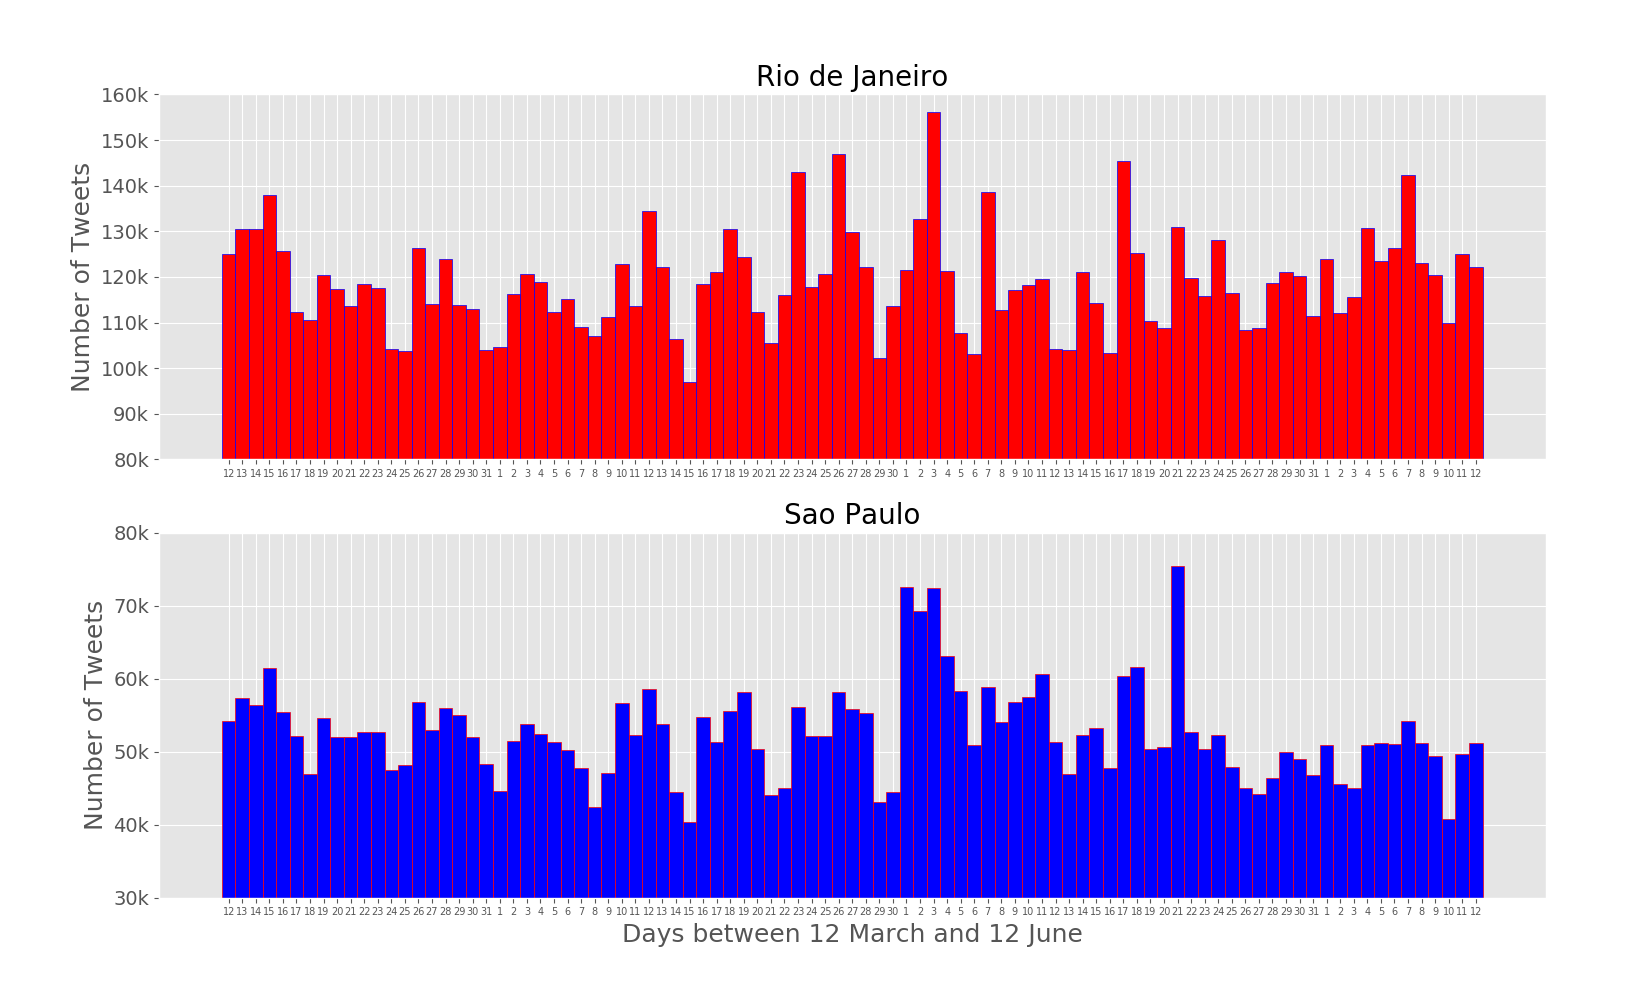
\includegraphics[width=\linewidth]{figures/rio_sp_whole_months.png}
   \caption{}
   \label{fig:portuguese_cities_whole_months} 
	\end{subfigure}

	\begin{subfigure}[t]{\textwidth}
    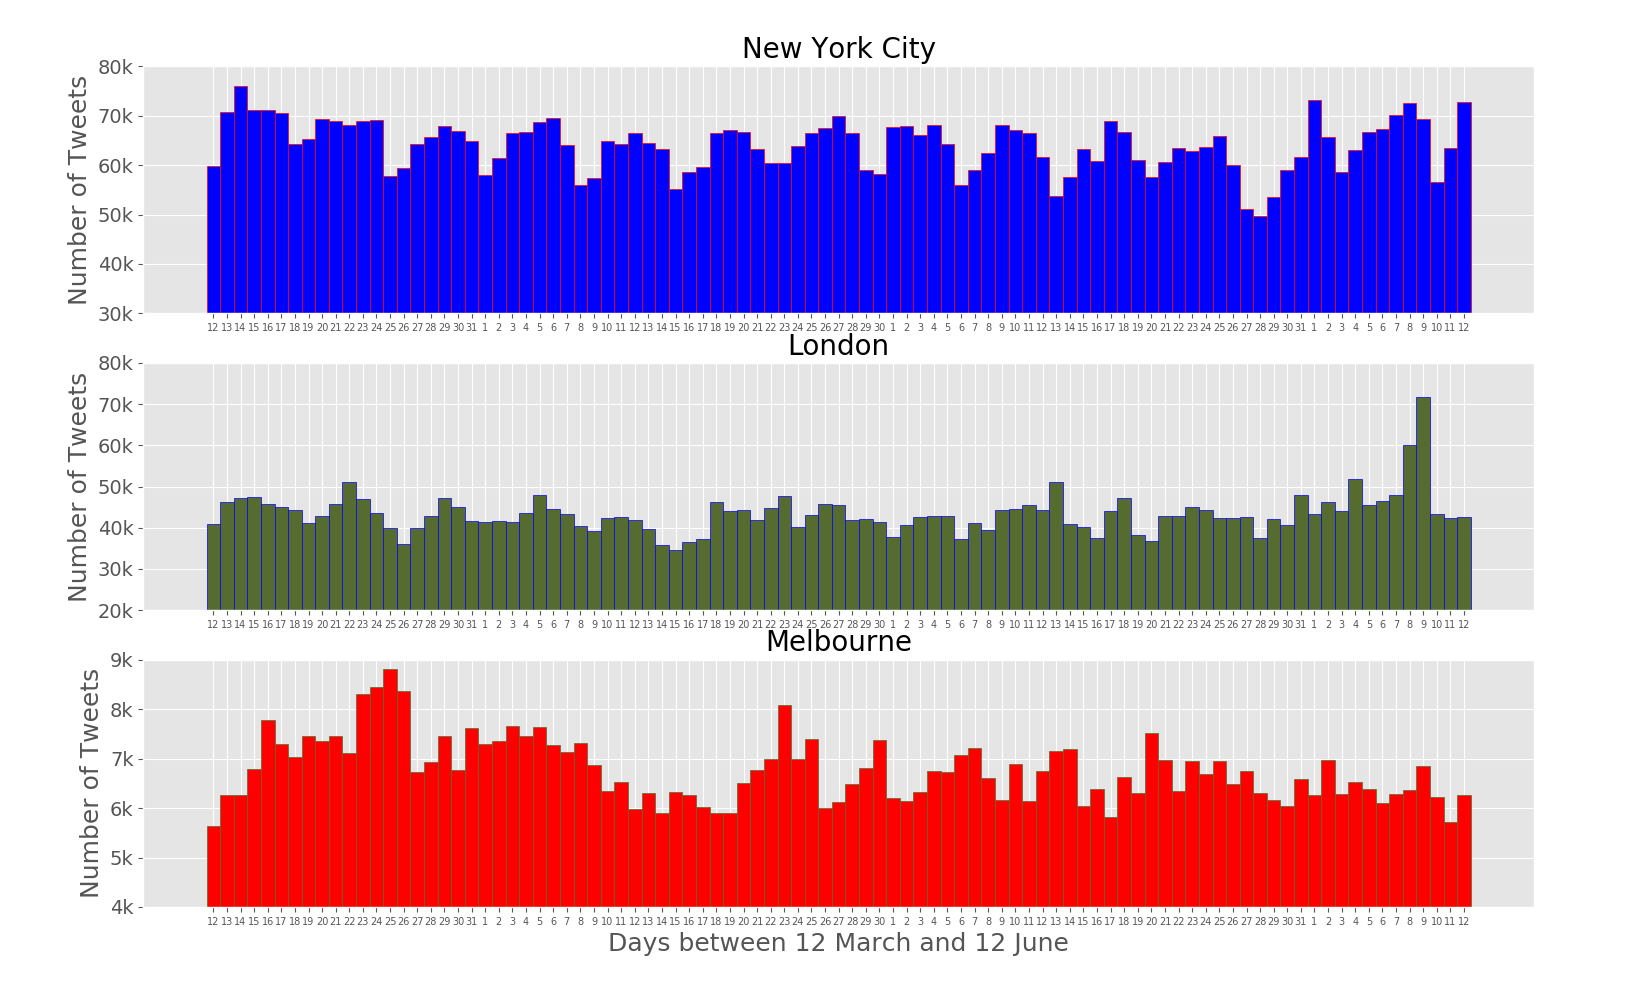
\includegraphics[width=\linewidth]{figures/nyc_london_melbourne_whole_months.png}
    \caption{}
    \label{fig:english_cities_whole_months}
	\end{subfigure}

\caption[Two numerical solutions]{(a) Rio de Janeiro and São Paulo - Portuguese Cities (b) New York City, London and Melbourne - English Cities}
\end{figure}

\subsection{Metadata Composition}

 Table~\ref{tab:entities} present the results for the \emph{entities} count and it is possible verify that \emph{urls} and \emph{user mentions} are most used ones over both datasets. Such information shows that users tend to tag another ones in a message meaning that tweets are used as a mean of communication.

\begin{table*}[!htbp]
\small
\centering
\caption{Datasets entities statistics}
\label{tab:entities}
\begin{tabular}{|c|c|c|c|c|c|l|c|l|}
\hline
\multirow{2}{*}{\textbf{City}} & \multicolumn{2}{c|}{\textbf{Hashtags (\#)}} & \multicolumn{2}{c|}{\textbf{User Mentions (@)}} & \multicolumn{2}{c|}{\textbf{URLs}} & \multicolumn{2}{c|}{\textbf{Media}} \\ \cline{2-9} 
 & \textbf{Total} & \textbf{\%} & \textbf{Total} & \textbf{\%} & \textbf{Total} & \textbf{\%} & \textbf{Total} & \textbf{\%} \\ \hline
\textbf{Rio de Janeiro} & 525,550 & 5\% & 1,340,334 & 13\% & 1,509,742 & 14\% & 389,864 & 4\% \\
\textbf{São Paulo} & 585,365 & 12\% & 1,072,566 & 22\% & 885,369 & 18\% & 302,579 & 6\% \\ \hline
\end{tabular}
\end{table*}

The grouping of tweets by the day of the week is illustrated in Figure~\ref{fig:box_plot_daily} and particular points can be observed and considered uncommon. For both cities distributions and with respect to geo-located tweets, Friday is the less active day while the major activity occurs in the first days of the week. This is a strange phenomenon since Friday is transition of the labour week days to the weekend and people could use more the microblog service to share their free time.

\section{Topic Modelling}\label{sec:topic_modeling}
This section is related to the experiment of automatically characterize tweets in two different Brazilian cities, Rio de Janeiro and São Paulo. We used an unsupervised learning approach to tackle the task of topic modelling in order to compare both cities and see if there are differences between subjects people talked about. Automatic characterization of text messages is a laborious and time consuming task since it is necessary to assure the right level of abstraction in the learning model; very much similarly to human minds, which essentially present a bounded rationality nature, our learning model needs to be trained in order to assimilate the necessary knowledge and perform the appropriate analogies so as to discover different topics within the tweets' contents. The premises to implement such a mechanism are presented and discussed in the following subsections.

\subsection{Data Selection}
The data selected to conduct this experiment is correspondent to a period of two months, between days March 12 and May 12, 2017. 

The resulting datasets sum up a total of 12.5M and 6.3M tweets for Rio de Janeiro and for São Paulo, respectively. Due to the problem detected in Section~\ref{sec:data_collection}, we filtered the data in order to only use the tweets that were actually inside the cities' areas. The final composition of the datasets is presented in Table~\ref{tab:datasets}, and the results of the filtering process shown that almost 6M tweets were not located inside the bounding-boxes of the cities.

\begin{table*}[ht]
\small
\centering
\caption{Datasets composition}
\label{tab:datasets}
\resizebox{\textwidth}{!}{\begin{tabular}{|c|c|c|c|c|c|c|}
\hline
\textbf{City}  & \textbf{All} & \textbf{PT} & \textbf{Non-PT} & \textbf{\begin{tabular}[c]{@{}c@{}}In \\ Bounding-Box\end{tabular}} & \textbf{\begin{tabular}[c]{@{}c@{}}Out\\ Bounding-Box\end{tabular}} & \textbf{\begin{tabular}[c]{@{}c@{}}PT and \\ In Bounding-Box\end{tabular}} \\ \hline
Rio de Janeiro & 12,531,000 & 10,570,000 & 1,961,000 & 8,644,000 & 3,886,000 & 7,353,000 \\ \hline
São Paulo & 6,352,000 & 4,886,000 & 1,466,000 & 4,247,000 & 2,105,000 & 3,313,000 \\ \hline
\end{tabular}}
\end{table*}

The subset of data composed by Portuguese tweets and located inside the cities' bounding-boxes was used to conduct the experiment described in this section. Such subset can be sum up to a total of 7.3M and 3.3M for Rio de Janeiro and São Paulo, respectively.

\subsection{Data Preparation}
Usually, to tackle topic modelling tasks in text documents it is required several pre-processing steps. Such pre-processing to the data helps the operations made by the LDA model, which is the technique used here. Removing unnecessary words, transforming words into their root form as so deleting all the punctuation are some of the common text mining pre-processing steps. Here, each tweet of both datasets was submitted to a required group of pre-processing operations in order to train a LDA model and proceed with the experiments. The pre-processing steps were the ones detailed below.

\begin{itemize}
\item \textbf{Lowercasing:} Every message presented in a tweet was converted into lower case;
\item \textbf{Cleaning Entities and Numbers:} Removing \textit{URLs}, user mentions, \textit{hashtags} and digits from the text message;
\item \textbf{Lemmatization:} Only plural words were transformed into singular ones;
\item \textbf{Transforming repeated characters:} Sequences of characters repeated more than three times were transformed, e.g. "loooool" was converted to "loool";
\item \textbf{Punctuation Removal:} Every punctuation was removed as well as smiles (e.g. \texttt{:)}, \texttt{:-)}, \texttt{=D}) or even \emph{emoticons};
\item \textbf{Stop Words Removal:} The removing of this kind of words was made using the Portuguese NLTK dictionary;
\item \textbf{Short Tokens Removal:} Words such as 'kkk', 'aaa', 'aff' and other of the same style were removed.
\end{itemize}

After the data preparation phase, 772,017 tweets have their message empty which conclude that its content was irrelevant for the final experiment phase.

\subsection{Features Selection}
Topic modelling requires, like in other learning model, a group of features to be trained. In this case, we used the Bag-of-Words representation matrix - which is a representation where each document is converted to a frequency vector according to the number of occurrences of each word in the message. The set of features was limit to a dictionary containing 10,000 words and it only took into account uni-grams in the message content. The dictionary was also limited to words that occur in a maximum percentage of 40$\%$ in the whole dataset, avoiding common words that were not removed because they were not included in the NLTK Stop Words list. The minimal occurrence value for a word being considered was set to 10.

\subsection{LDA Model Parametrization}
In order to understand and see the LDA model performance, we set five different numbers for the topics results parameter of the training process: 5, 10, 20, 25 and 50 topics, being this the one with better results. The number of iterations to train the model was set to 20, since our desired was to reproduce the experiment made by G. Lansley et al.~\cite{lansley2016geography} to the city of London. Finally but not the least, each tweet in the datasets was treated as a single document comprehending that, in total, 6,580,983 different documents were used in the model training process. The complete pipeline according to all the steps taken to conduct this experiment is observable in Figure~\ref{fig:pipeline_lda}.

\begin{figure}[h]
\centering
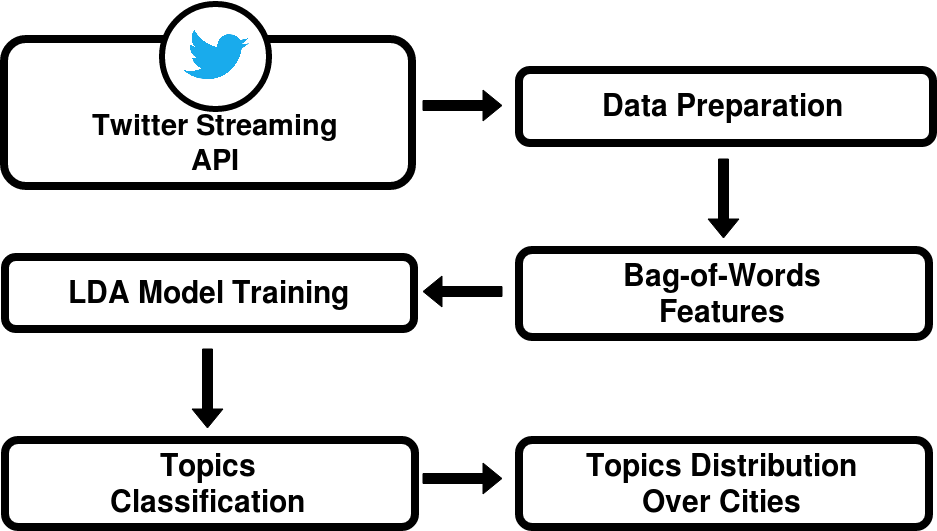
\includegraphics[width=0.6\linewidth]{figures/pipeline_lda.png}
\caption{Correspondent pipeline of the topic modelling experiment}
\label{fig:pipeline_lda}
\end{figure}

\subsection{Results and Analysis}
To evaluate the experimental results obtained for each model (where the difference underlies on the variation of the number of topics), a list with the most frequent 50 words for each topic was extracted. In Table~\ref{tab:topics_classification} we can observe a sample (20 top words) selected out of the 50 studied. Nonetheless, the final evaluation takes into consideration the 50 frequent words.

\begin{table}[h]
\centering
\caption{Example of the topics classification}
\label{tab:topics_classification}
\resizebox{\textwidth}{!}{\begin{tabular}{c|c}
\hline
\textbf{\begin{tabular}[c]{@{}c@{}}Words\\ (only 20 words)\end{tabular}} & \textbf{\begin{tabular}[c]{@{}c@{}}Topic\\ Classification\end{tabular}} \\ \hline
\begin{tabular}[c]{@{}c@{}}paulo, vai, hoje, dia, jogo, ser, melhor, time, vamo, brazil, \\ todo, santo, brasil, gol, cara, aqui, agora, corinthiam, ano, palmeiro, vem, ...\end{tabular} & \begin{tabular}[c]{@{}c@{}}Sports and\\ Games\end{tabular} \\ \hline
\begin{tabular}[c]{@{}c@{}}vou, dia, dormir, queria, hoje, ficar, casa, semano, quero, ter, \\ ainda, hora, agora, sono, aula, acordar, acordei, cedo, fazer, prova, ...\end{tabular} & \begin{tabular}[c]{@{}c@{}}Wake-up\\ Messages\end{tabular} \\ \hline
\begin{tabular}[c]{@{}c@{}}top, social, artist, vote, the, award, army, bom, voting, doi, \\ bogo, oitenta, sipda, today, vinte, prepara, cypher, oito, quatro, man, ...\end{tabular} & \begin{tabular}[c]{@{}c@{}}Voting and\\ Numbers\end{tabular} \\ \hline
\begin{tabular}[c]{@{}c@{}}marco, nada, falar, emilly, gente, quer, nao, pessoa, nunca, fala, \\ vai, falando, sobre, chama, agora, manda, vem, mensagem, vivian, bbb, ...\end{tabular} & \begin{tabular}[c]{@{}c@{}}Big Brother\\ Brazil 2017\end{tabular} \\ \hline
\begin{tabular}[c]{@{}c@{}}paulo, brazil, sao, santo, vila, just, parque, posted, photo, shopping, \\ paulista, centro, bernardo, jardim, cidade, avenido, praia, santa, campo, academia\end{tabular} & \begin{tabular}[c]{@{}c@{}}Tourism and\\ Places\end{tabular} \\ \hline
\end{tabular}}
\end{table}

We also selected and manually analyse a random sample (with the size of 200) of tweets for each topic. This sampling was done in order to get better consistency and trustiness about the classification and characterization of the tweets.

It was found a group of 50 topics which had the largest number of distinct topics between them. However, there were topics which theme was the same (e.g. Love and Romance Problems or Brazilian Football \textit{versus} European Football). Within this, such groups were aggregate into the same topic, \textit{Relationships} and \textit{Sports and Games}, respectively. After this grouping process, a total of 29 different topics was achieved. 

Some tweets that have added complexity to our classification objective, such as, for example, "\textit{queria namorar um mano parecido com o josh}" (Relationship) and "\textit{como eu queria meus amigos aqui agora cmg}" (Friendship), raised some doubts about which topic this tweets may belong: Relationship, Friendship or even Actions or Intentions. In a perspective of context, the first tweet belongs to the theme \texttt{flirt}, which is directly related to Relationship. The theme on the second tweet is missing the company of friends, i.e. conviviality, which is related to Friendship. The decision of join the two topics was due to the proximity between them which have as content both types of tweets, talking about love/relationship and friendship, and with this in consideration both topics should be aggregated in order to assure the desired consistency in the classification.

The final set of topics (50 topics) to be considered was selected accordantly to the most recurring subjects. The final classification and details associated with the whole dataset for each city is presented in Table~\ref{tab:final_classification}. Almost every topics demonstrated a balanced distribution, with exception of \textit{Relationships and Friendship} and \textit{Personal Feelings} for Rio de Janeiro and São Paulo, respectively. The difference that appear in this topics is a consequence of the final grouping process, since there was a considerable number of words been shared among this topics. This issue complicated our classification task, compelling to an high amount of undesired aggregations.

\begin{table}[ht]
\small
\caption{Final results of the LDA topics aggregation}
\label{tab:final_classification}
\resizebox{\textwidth}{!}{\begin{tabular}{l|cc|cc|c}
\hline
\multicolumn{1}{c|}{\multirow{2}{*}{\textbf{Topic Group}}} & \multicolumn{2}{c|}{\textbf{Rio de Janeiro}} & \multicolumn{2}{c|}{\textbf{São Paulo}} & \multicolumn{1}{c|}{\multirow{2}{*}{\textbf{Diff (\%)}}} \\ \cline{2-5}
\multicolumn{1}{c|}{} & \textbf{No. Tweets} & \textbf{Percentage (\%)} & \textbf{No. Tweets} & \textbf{Percentage (\%)} & \multicolumn{1}{c|}{} \\ \hline
Academic Activities & 101,590 & 1,54\% & 90,616 & 3,30\% & -1,76\% \\
Actions or Intentions & 600,030 & 9,12\% & 128,710 & 4,69\% & \textbf{+4,43\%} \\
Antecipation and Socialising & 132,606 & 2,01\% & 0 & 0,00\% & \textbf{+2,01\%} \\
BBB17 & 122,054 & 1,85\% & 68,385 & 2,49\% & -0,64\% \\
Body, Appearances and Clothes & 160,342 & 2,44\% & 71,447 & 2,60\% & -0,17\% \\
Food and Drink & 167,204 & 2,54\% & 58,407 & 2,13\% & +0,41\% \\
Health & 119,013 & 1,81\% & 0 & 0,00\% & \textbf{+1,81\%} \\
Holidays and Weekends & 104,695 & 1,59\% & 79,610 & 2,90\% & -1,31\% \\
Informal Conversations & 272,502 & 4,14\% & 138,848 & 5,06\% & -0,92\% \\
Live Shows, Social Events and Nightlife & 359,342 & 5,46\% & 140,240 & 5,11\% & +0,35\% \\
Mood & 139,287 & 2,12\% & 138,399 & 5,04\% & \textbf{-2,92\%} \\
Movies and TV & 285,198 & 4,33\% & 39,778 & 1,45\% & \textbf{+2,89\%} \\
Music and Artists & 84,407 & 1,28\% & 78,142 & 2,85\% & 1,56\% \\
Negativism, Pessimism and Anger & 229,104 & 3,48\% & 183,050 & 6,67\% & \textbf{-3,18\%} \\
Numbers, Quantities and Classification & 86,897 & 1,32\% & 78,160 & 2,85\% & -1,53\% \\
Optimism and Positivism & 106,714 & 1,62\% & 39,725 & 1,45\% & +0,18\% \\
Personal Fellings & 375,735 & 5,71\% & 532,331 & 19,38\% & \textbf{-13,67\%} \\
Politics & 81,254 & 1,23\% & 46,758 & 1,70\% & 0,47\% \\
Relationships and Friendship & 1,524,804 & 23,17\% & 187,541 & 6,83\% & \textbf{+16,34\%} \\
Religion & 183,174 & 2,78\% & 66,788 & 2,43\% & +0,35\% \\
Routine Activities & 334,216 & 5,08\% & 82,421 & 3,00\% & +2,08\% \\
Slang and Profinities & 241,676 & 3,67\% & 44,620 & 1,62\% & +2,05\% \\
Social Media Applications & 105,809 & 1,61\% & 44,073 & 1,60\% & +0,01\% \\
Sport and Games & 382,479 & 5,81\% & 133,047 & 4,84\% & +0,97\% \\
Tourism and Places & 59,288 & 0,90\% & 86,519 & 3,15\% & -2,25\% \\
Transportation and Travel & 130,261 & 1,98\% & 63,923 & 2,33\% & -0,35\% \\
Weather & 91,302 & 1,39\% & 42,588 & 1,55\% & -0,16\% \\
Shopping & 0 & 0,00\% & 44,470 & 1,62\% & \textbf{-1,62\%} \\
Voting & 0 & 0,00\% & 37,687 & 1,37\% & \textbf{-1,37\%} \\ \hline
\end{tabular}}
\end{table}

Additionally to the manual verification of a sample of tweets for each topic, we also produced a temporal week day distribution,  with the objective to observe if some topics had more mentions in certain days than others.

For making such observations some assumptions were made in relation with some \textit{hot} topics. More specifically, we think that is valid to assume that people will talk more about \textit{Religion} in the weekend, since they go to the church in those days. The same result is likely to happen for topics like \textit{Holidays and Weekends} or \textit{Sports and Games}, since events related to this thematics occur during specific time-frames. 

Only 12 topics of the finals 29 were selected for this part of the study, predicting them and comparing the final results, such as, but not limited to, \textit{Sports and Games}, \textit{Religion}, \textit{Holidays and Weekends}, \textit{Movies and TV}, \textit{Live Shows, Social Events and Nightlife}. The temporal distribution is showed in Figure~\ref{fig:topics_heat_maps} as a heat map, where each row is independent from the others.

The necessity of applying such restrictions is due to the need of seeing in which days each topic is more talked about. For both cities the topic \textit{Sports and Games} is more mentioned in Tuesdays and Saturdays. Indeed, this observation correlates with the days that topic-related events happens. Namely, Tuesdays and Wednesday correspond to the days when the \textit{UEFA Champions League} competition happens and Saturdays and Sundays to the days of \textit{Brazilian Football League} games. \textit{Holidays and Weekends} was a topic with interesting results regarding the temporal distribution, presenting Sundays as the day where more people talk about it. 

Furthermore, it is worth mentioning that our model had successfully discover a topic related to Big Brother Brazil 2017 (BBB17), a well-known reality show. The amount of geo-located tweets concerning this topic was considerable (1.85\% and 2.49\%, in RJ and SP, respectively), rising the question about what led people to geo-located them in such topic.

\begin{figure}[h]
\centering
\begin{subfigure}{0.49\textwidth}
\centering
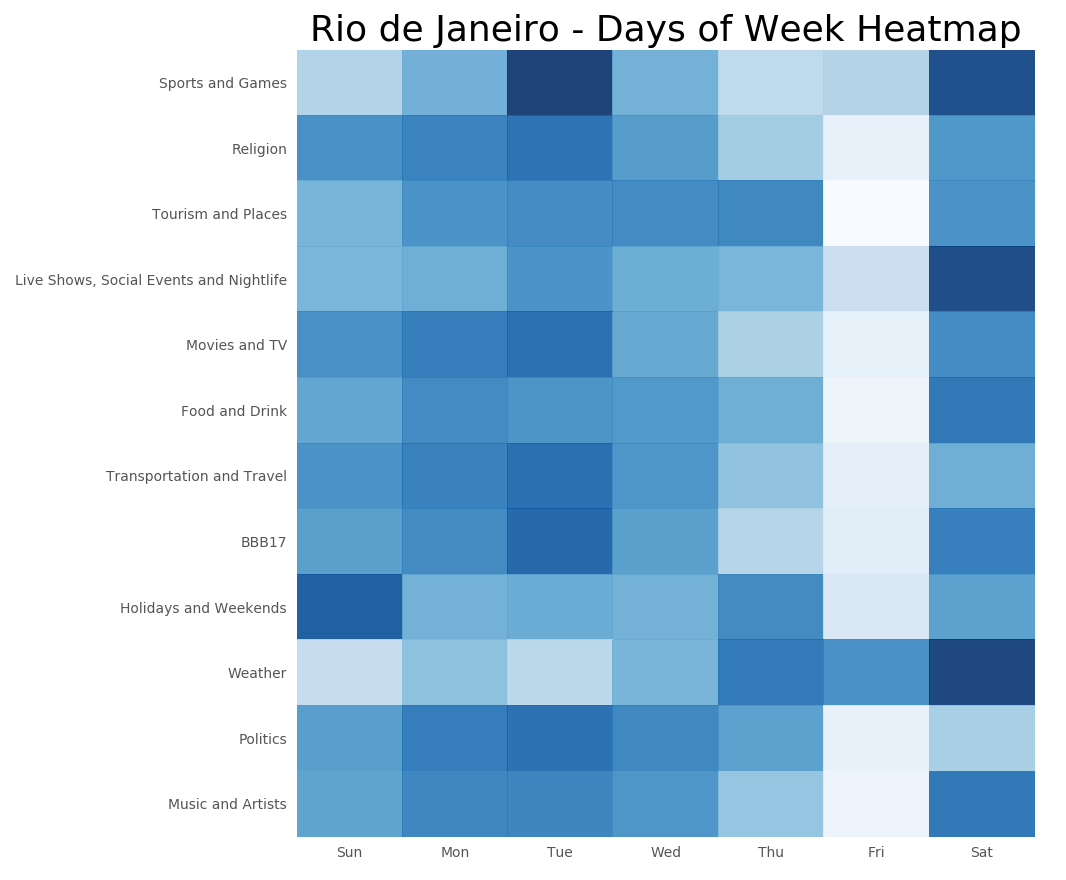
\includegraphics[width=1.0\linewidth]{figures/rio_topics_heatmap.png}
\label{fig:rio}
\end{subfigure}
\begin{subfigure}{0.49\textwidth}
\centering
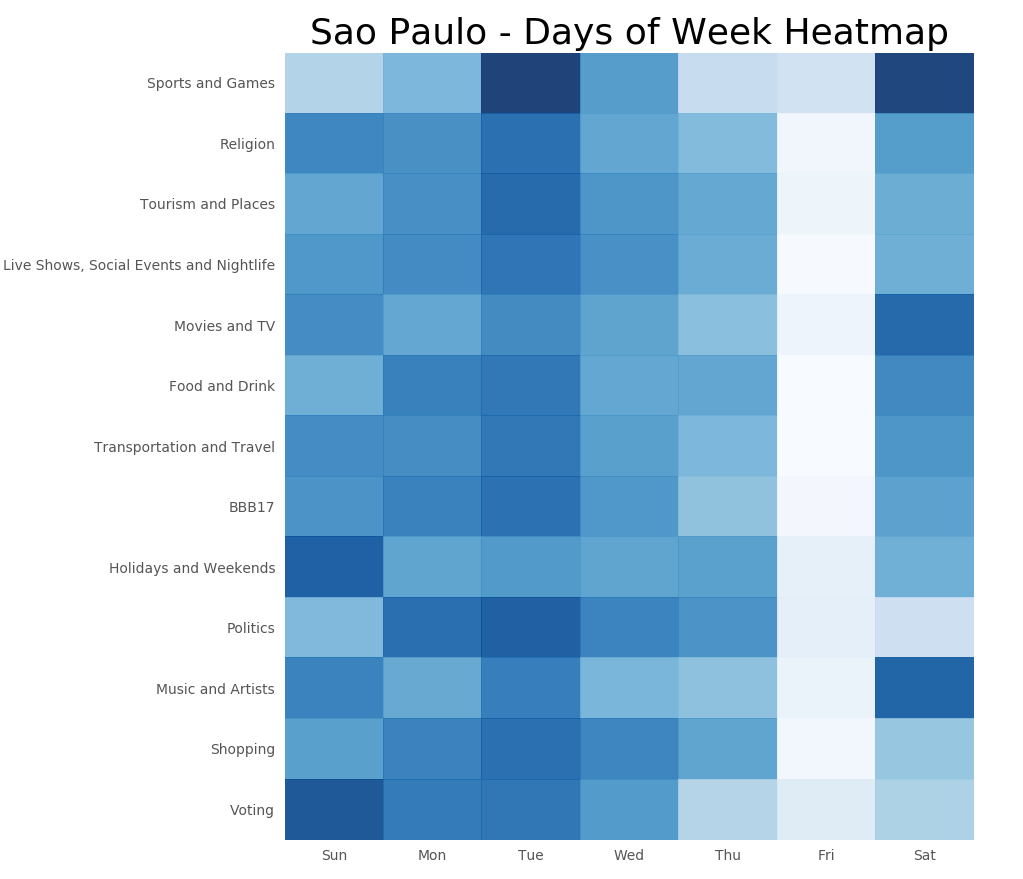
\includegraphics[width=1.0\linewidth]{figures/sp_topics_heatmap.png}
\label{fig:sp}
\end{subfigure}
\caption{Day-of-the-week activity per each topic in both cities, Rio de Janeiro and São Paulo}
\label{fig:topics_heat_maps}
\end{figure}

\subsection{Final Remarks}
The methodology reported across this experiment is concerned with topic modelling over two datasets from two Brazilian cities in order to characterize the topics that people talked about and compare the results in both scenarios. LDA models usually requires documents of large size, or at least more complex than a single tweet, in order to get good performance. A traditional approach was followed considering each tweet as a document instead of trying aggregate tweets in more complex documents taking into consideration some criteria, e.g. grouping by date and hour. The final results showed that topics in both cities are very similar and only two of them are unique. With exception of topics - \textit{Relationships and Friendship} and \textit{Personal Feelings}, the percentage difference between similar topics was comprehended in the interval 0.16-4.43\% evidencing the fact that both cities are similar besides the different factors that characterize each one: population, culture, lifestyle and also the region where the city is located in. Although all this analysis, we can not assure that inside a topic we do not have more topics hidden. Our classification was limited to the verification of the 50 top words and the manually verification of a sample of 200 tweets since the resulting amount of tweets for each topic is impossible to verify one by one. Due to this, another classification approach need to be explored and a promising one was proposed by D. Ramage et al.~\cite{ramage2010characterizing}. The classification will be automatic by adding a supervised extra layer to the pipeline. However, to assure trustiness in the results the data may be manually labelled for the training phase of the model classification or, at least, have reliable sources, for example, exploring the topics provide by the Wikipedia articles\footnote{\url{https://dumps.wikimedia.org/ptwiki/20170601/}}.

\section{Travel-related Classification}\label{sec:travel_related_classification}
The main goal of this section is to detail the experiment that supports the characterization of travel-related tweets in Rio de Janeiro and in São Paulo. Considering the volume of the collected data, it was then necessary to automatically identify tweets whose content somehow suggests to be related to the transportation domain. Conventional approaches would require us to specify travel-related keywords to classify such tweets. On the contrary, our approach consisted in training a classifier model to automatically discriminate travel-related tweets from non-related ones. 

One big challenge always present in text analysis is the sparse nature of data, which is especially the case in Twitter messages.
Conventional techniques such as Bag-of-Words tend to produce sparse representations, which become even worse when data is composed by informal and noisy content.

Word embeddings, on the other hand, is a text representation technique that tries to capture syntactic and semantic relations from words. The result is a more cohesive representation where similar words are represented by similar vectors. For instance, \emph{"taxi"/"uber"}, \emph{"bus/busão/ônibus"}, \emph{"go to work"/"go to school"} would yield similar vectors respectively.
We are particularly interested in exploring the characteristics of word embeddings techniques to understand which extent it is possible to improve the performance of our classifier to capture such travel-related expressions. In the following subsections, we describe the necessary steps to build our classification model.

\subsection{Data Preparation}
Each tweet of our training and test sets was submitted to a small and basic group of pre-processing operations, as detailed below.

\begin{itemize}
\item \textbf{Lowercasing:} Every message presented in a tweet was converted into lower case;
\item \textbf{Transforming repeated characters:} Sequences of characters repeated more than three times were transformed, e.g. "loooool" was converted to "loool";
\item \textbf{Cleaning:} URLs and user mentions were removed from the text.
\end{itemize}

\subsection{Features Selection}\label{features_4_3_2}
We established the use of different groups of features to train our classification model, namely bag-of-words, bag-of-embeddings - word embeddings dependent technique - and both combined. Such groups are detailed below.

\begin{itemize}
\item \textbf{Bag-of-words (BoW):} This group of features was obtained using unigrams with standard bag-of-words techniques. We considered the 3,000 most frequent terms across the training set excluding the ones found in more than 60$\%$ of the documents (tweets);

\item \textbf{Bag-of-embeddings (BoE):} We applied bag-of-embeddings to each tweet using a \textit{doc2vec} model~\footnote{\url{https://radimrehurek.com/gensim/models/doc2vec.html} (last visited on 9 June, 2017)} combining Deep Learning and \textit{paragraph2vec}. The model was trained with 10 iterations over the whole Portuguese dataset using a context window of value 2 and feature vectors of 100 dimensions. We then took the corresponding embedding matrix to yield the group of features fed into our classification routine. 

\item \textbf{Bag-of-words plus Bag-of-embeddings:} We horizontally combined both the above matrices into a single one and used it as a single group of features.
\end{itemize}

\subsection{Training and Test Datasets}
The construction of the training and test sets followed a traditional approach. We thus tried to select balanced training sets, to which it was necessary to identify tweets that could possibly be travel-related.
We were inspired by a strategy used in the study by Maghrebi~et~al.~\cite{maghrebi2016transportation}, which consists in searching tweets from a collection using specific travel terms and regular expressions. Using the terms declared in Table~\ref{terms} combined with the regular expression $space + term + space$, we found about 30,000 tweets. From this subset, we randomly selected a small sample of 3,000 tweets to manually confirm if they were indeed related to travel topics. After this manual annotation we selected 2,000 tweets and used them as positive samples in the training dataset.

In order to select negative samples for the training dataset we randomly selected 2,000 tweets and also manually verified their content to assure that they were not travel-related. Finally, our training set was composed by 4,000 tweets, from which 2,000 were travel-related and 2,000 were not. 
We selected 1,000 tweets randomly that were not present in the training set to build the test set, and then manually classified them as travel-related or non-travel-related. In the end, 71 tweets were found to be travel-related and whereas 929 were not.

\begin{table}[!htbp]
\centering
\caption{Travel terms used to build the training set}
\label{terms}
\begin{tabular}{c|c}
\hline
\textbf{Mode of Transport} & \textbf{Terms} \\ \hline
Bike & bicicleta, moto \\
Bus & onibus, ônibus \\
Car & carro \\
Taxi & taxi, táxi \\
Train & metro, metrô, trem \\
Walk & caminhar \\ \hline
\end{tabular}
\end{table}

\subsection{Estimators and Evaluation Metrics}
Support Vector Machines (SVM), Logistic Regression (LR) and Random Forests (RF) were the classifiers used in our experiments. The SVM classifier was tested under three different kernels, namely \textit{rbf}, \textit{sigmoid} and \textit{linear}; the latter proved to obtain the best results. 

The LR classifier was used with the standard parameters, whereas the RF classifier used 100 trees in the forest. The gini criterion and the maximum number of features were limited to those as aforementioned in Section~\ref{features_4_3_2}, in the case of the RF classifier.

To evaluate the performance of the classifiers in our experiences we used five different metrics. Firstly we compute a group of three per-class metrics, namely precision, recall and the F1-score. Bearing in mind this study considers a binary classification, metrics were associated with the travel-related class only, i.e. the positive class. Therefore, the interpretation for each metric is provided below:

\begin{itemize}
\item \textbf{Precison:} Represents the fraction of correct predictions for the travel-related class (Equation~\ref{eq:precision}).

\item \textbf{Recall:} Represents the fraction of travel-related tweets correctly predicted (Equation~\ref{eq:recall}).
\begin{multicols}{2}
	\begin{equation}\label{eq:precision}
		Precision = \frac{tp}{tp+fp}
    \end{equation}
    
	\begin{equation}\label{eq:recall}
		Recall = \frac{tp}{tp+fn}
	\end{equation}
\end{multicols}

where \textbf{$tp$} is related to the true positives classified tweets, \textbf{$fp$} represents the false positives and \textbf{$fn$} are the false negatives.

\item \textbf{F1-score:} Represents the harmonic mean of precision and recall.
\end{itemize}

\begin{equation}
{F1}_{score} = 2*\frac{precision*recall}{precision+recall}
\end{equation}

Once these first three metrics only showed us the performance of the classifier for a discrimination threshold of 0.5, we decided to calculate another metric. The ROC (Receiver operating characteristic) curve gives us the TPR (True positive rate) and the FPR (False positive rate) for all possible variations of the discrimination threshold. Through the ROC curve, we compute the area under the curve (AUC) to see what was the probability of the classifier to rank a random travel-related tweet higher than a random non-related one.

\subsection{Results and Analysis}
Table~\ref{classifiers} presents the results obtained using the different features combination for our test set composed by 1,000 tweets manually annotated. According to the evaluation metrics we conclude that the bag-of-word and bag-of-embeddings combined produced better classification models. The model produced by the Linear SVM performed slightly better than the LR and the RF. Interesting to note is that BoW features have influence on the precision scores obtained from our results, producing more conservative classifiers. Regarding the recall results, we can see that the Logistic Regression using only bag-of-embeddings features was the model with best results; perhaps if the precision is taken into consideration, the same conclusions will not be possible. Analysing the scores provided in Table~\ref{classifiers}, the best model under the F1-score was the Linear SVM, with a score of 0.85.

\begin{table}[!htbp]
\footnotesize
\centering
\caption{Classifiers Experiences}
\label{classifiers}
\begin{tabular}{|c|c|c|c|c|}
\hline
\textbf{Classifier}                  & \textbf{Features} & \textbf{Precision} & \textbf{Recall} & \textbf{F1-score} \\ \hline
\multirow{3}{*}{Linear SVM}          & BoW               & 1.0                & 0.6761          & 0.8067            \\
                                     & BoE               & 0.4338             & 0.8309          & 0.5700            \\
                                     & BoW + BoE         & \textbf{1.0}       & \textbf{0.7465} & \textbf{0.8548}   \\ \hline
\multirow{3}{*}{Logistic Regression} & BoW               & 1.0                & 0.6338          & 0.7759            \\
                                     & BoE               & 0.4444             & 0.8451          & 0.5825            \\
                                     & BoW + BoE         & 1.0                & 0.6761          & 0.8067            \\ \hline
\multirow{3}{*}{Random Forest}       & BoW               & 1.0                & 0.6338          & 0.7759            \\
                                     & BoE               & 0.2298             & 0.8028          & 0.3574            \\
                                     & BoW + BoE         & 1.0                & 0.6338          & 0.7759            \\ \hline
\end{tabular}
\end{table}

The performance of all three classifiers is illustrated using the ROC Curve in Fig. \ref{fig:roc_curve}. The area under the curve of the Receiver Operating Characteristic (AUROC) was very similar for both the Logistic Regression and the Linear SVM models. The results obtained from the Random Forest model were not so promising as expected.

\begin{figure}[!htbp]
  \caption{ROC Curve of SVM, LR and RF experiences}
  \centering
  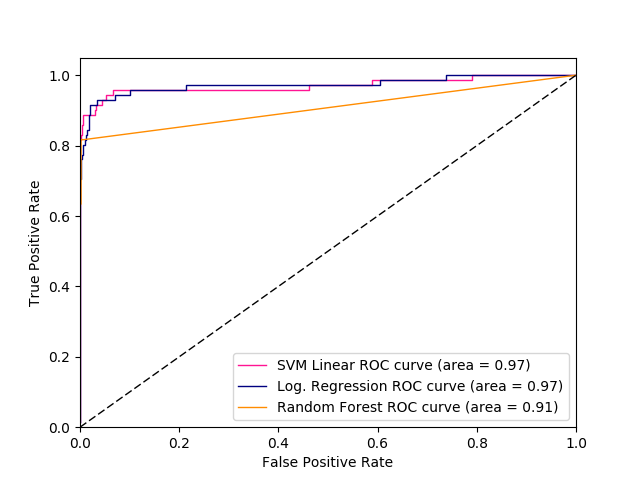
\includegraphics[width=0.7\textwidth]{figures/roc_auc_brazilian_travel_related}
  \label{fig:roc_curve}
\end{figure}

After the selection of our classification model, we decided to classify all the Portuguese dataset and draw some statistics from the results. The trained Linear SVM classifier was used to predict whether tweets were travel-related or not, since it was the model presenting the best score under the F1-score metric (as shown in Table~\ref{classifiers}). From a total of 7.8M tweets, our classifier was able identified 37,300 travel-related entries.

Fig.~\ref{predicted} depicts the distribution of travel-related tweets over the days of the week. We can see that the first three business days (Monday, Tuesday and Wednesday) are the ones on which the Twitter activity is higher for both cities in our study.

\begin{figure}[!htbp]
  \caption{Positive Predicted Tweets per Day of Week}
  \centering
    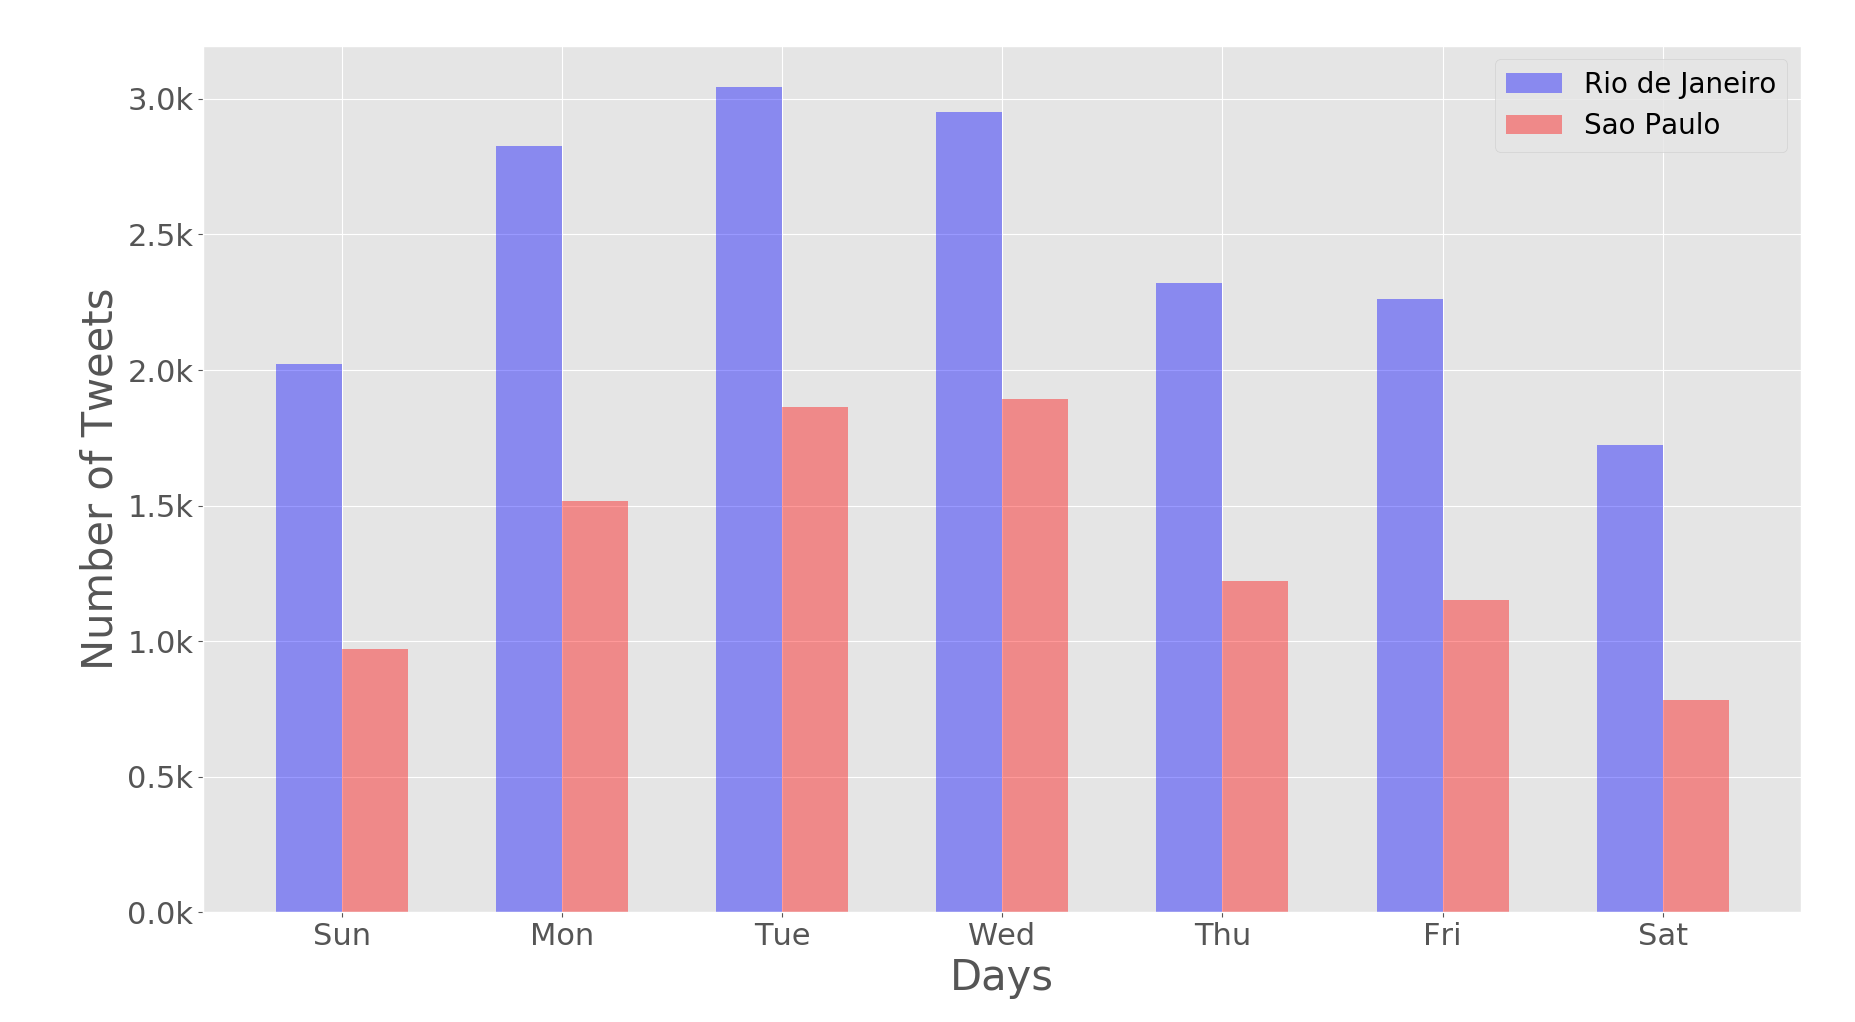
\includegraphics[width=0.7\textwidth]{figures/predicted_day_of_week}
    \label{predicted}
\end{figure}

\begin{figure}[!htbp]
  \caption{Rio de Janeiro Heatmap to the positive tweets}
  \centering
    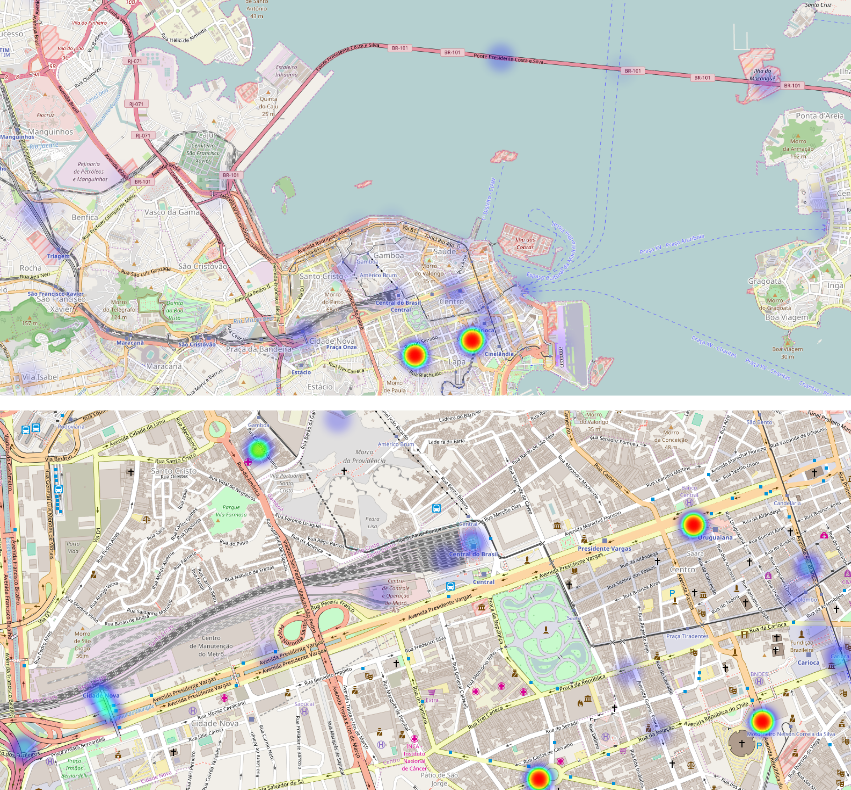
\includegraphics[width=0.725\textwidth]{figures/rio_1}
    \label{rio_heatmap}
\end{figure}

\begin{figure}[h]
  \caption{São Paulo Heatmap to the positive tweets}
  \centering
    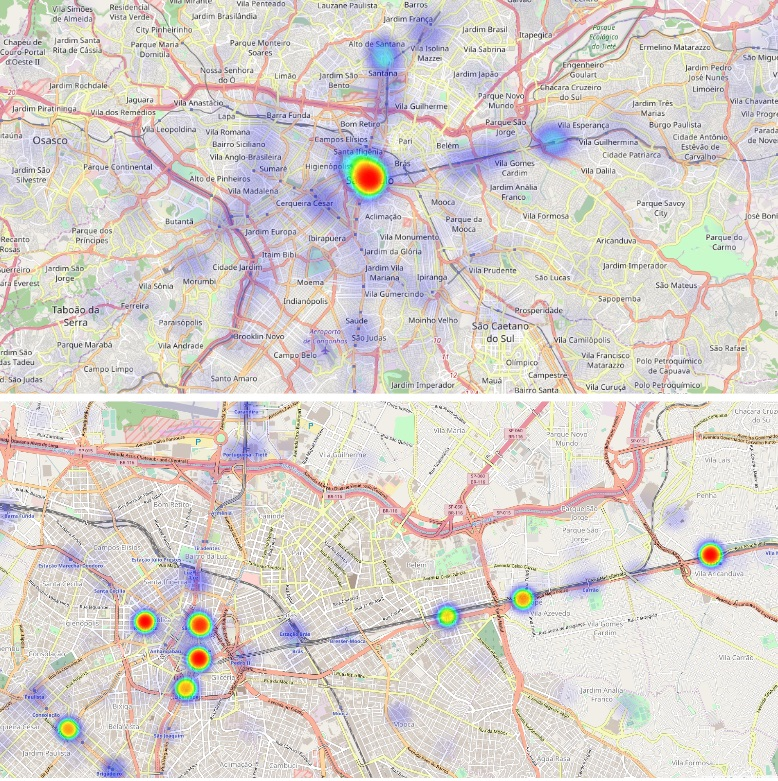
\includegraphics[width=0.725\textwidth]{figures/sp_1}
    \label{sp_heatmap}
\end{figure}

In order to understand the spatial distribution of travel-related tweets we generated a heatmap for both cities. From the heatmap of RJ, illustrated in Fig.~\ref{rio_heatmap}, it is possible to identify that some agglomerations of tweets are located at Central do Brasil, Cidade Nova and Triagem train stations, as well as at Uruguaiana, Maracanã and Carioca metro stations. The Rio-Niterói bridge, connecting Rio de Janeiro to Niterói, as well as the piers on both sides also presented considerable clouds of tweets classified as travel-related.

The heatmap for the city of SP, illustrated in Fig.~\ref{sp_heatmap}, was also an interesting case to observe. Almost every agglomeration matched some metro or train station. Estação Brás, Tatuapé, Belém, Estação Paulista, Sé, Liberdade were some of the stations highlighted in the heatmap. We could also identify a little agglomeration of travel-related tweets at Congonhas airport, even though no tweets seemed to mention the word \textit{plane} explicitly in the training of our classification model.

\subsection{Final Remarks}

\section{Travel-mode Extraction}\label{sec:travel_mode_extraction}
